\documentclass[00_mcda_tutorial.tex]{subfiles}

\begin{document}
\section*{Tutorial 4: sensitivity analysis}
\addtocounter{section}{1}
\addcontentsline{toc}{section}{\protect\numberline{}Tutorial 4: sensitivity analysis}

MCDA requires exact preference weights. However, in most benefit-risk assessment situations such exact weights are not available; they might lie on a range or simply be unknown. Further, the supplied data might have significant variance. In this tutorial we will investigate several ways to determine how sensitive the results of analyses are to such uncertainties.

\subsection*{Subjects covered}
\begin{itemize}
    \item Uncertainty in data and preferences
    \item Deterministic sensitivity analysis
    \item Stochastic sensitivity analysis
\end{itemize}

\noindent \faExclamationTriangle \, Note that this tutorial continues from the simplified version of the \href{https://www.ema.europa.eu/en/medicines/human/EPAR/zinbryta#authorisation-details-section}{Zinbryta assessment} used in the previous tutorial about benefit-risk analysis. At several points during this tutorial we ask you to compare results to those of the previous one, so it is helpful to have your work from the previous tutorial open in a separate browser tab or window.

\subsection*{Sign in to your organisation's ADDIS/MCDA.}
\leftpointright \, Open your browser and navigate to \href{https://mcda.drugis.org}{https://mcda.drugis.org}.
Use your Google account to sign in.

\begin{sidebar*}
In case of the enterprise edition, navigate to the URL provided by your organisation. Use your username and password to sign in.
\end{sidebar*}

You will be redirected to your personal homepage, containing your previously created workspaces, both finished and unfinished (if any).

\subsection*{Create the example workspace}
\leftpointright \, Click the ‘Create workspace’ button. In the dialog that appears, switch to 'Select tutorial workspace' and choose the ‘Zinbryta initial assessment simplified, stochastic’ option. You should now be on the Overview screen of a fresh workspace. Open the settings dialog and switch the ‘Measurements display mode’ to ‘'Values used in SMAA'’. Note the point estimates have confidence intervals for all measurements. To see which distributions these confidence intervals are based on, switch the measurements display to 'Entered distributions.'
\newline

\noindent \faGraduationCap \, For this tutorial example, we indicated explicitly when entering the data that we assume they are approximately normally distributed for their given point estimate and confidence interval (see Figure 3 in the first tutorial). This lets their distributions be used to perform stochastic sensitivity analysis, as explained towards the end of this tutorial.
\newline

\noindent \leftpointright \, Click on the ‘Problem definition’ tab. Consider how the confidence intervals for each criterion’s measurements are connected to the ‘Observed Range’ column in the scale ranges table.
\newline

\noindent \faGraduationCap \, The scale ranges for each criterion determine which highest and lowest values to consider when defining their partial value functions. Scale ranges can be wider than the observed data, but never narrower. If the data include uncertainty the confidence intervals are included in the scale ranges.

\subsection*{Deterministic sensitivity analysis}
\noindent \leftpointright \, Click on the ‘Preferences’ tab and define your partial value functions, as in our previous tutorial on benefit-risk analysis. Remember that lower is better for all criteria in this analysis. Note that the X-axis of each pvf corresponds to the scale range for that criterion.
\newline

\noindent \leftpointright \, Perform an ordinal ranking, with ARR most important, and the AEs in decreasing importance from top to bottom. Go to the 'Deterministic results' tab, and look at the 'Value profiles' plot. Compare it to the 'Value profiles' plot of the previous tutorial’s ordinal ranking scenario. Note that both alternatives derive some value from each criterion. Also note that now that uncertainty is included, Daclizumab actually has higher value.
\newline

\noindent \faGraduationCap \, Widening the scale ranges of your criteria is one way of incorporating uncertainty in your analyses. Since the partial value function for a criterion by definition returns an extreme value (either 0 or 1) at the minimum or maximum value of the scale range, measurements at these extremes will therefore have either maximally positive or maximally negative value. If you widen your scale ranges so that your measurements are never at these extreme ends, they will always have some positive contribution to that alternative’s value.
\newline

\noindent \leftpointright \, Let’s see what happens if we want to consider the case where the point estimate for ARR is too high for IFN $\beta$-1a 30$\mu$g. Click on this value in the effects table at the top of the page, and change it to approximately 0.353: the lowest value within the 95\% C.I. (Figure \ref{fig:changeARR}). Click the ‘Recalculate value profiles’ button below the effects table, and take a look at the new results. As it turns out, this single change is not sufficient to change the benefit-risk balance.
\newline

\begin{figure}[!h]
    \centering
    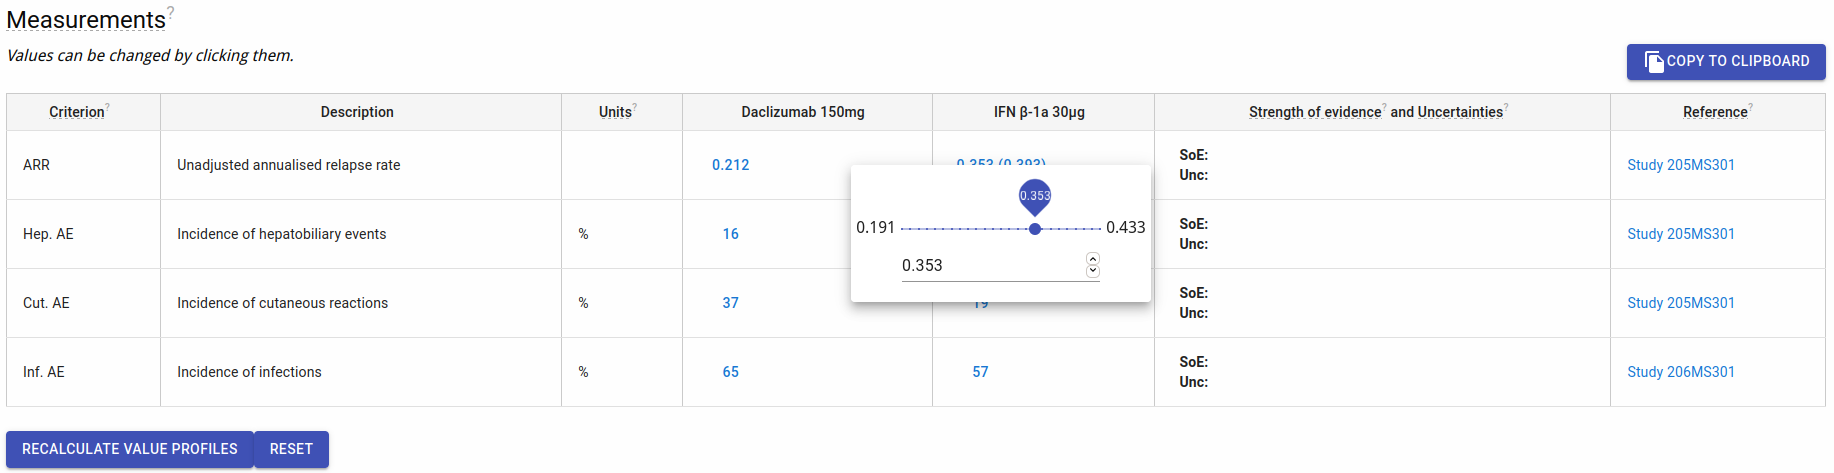
\includegraphics[width=\textwidth]{fig/changeARR.png}
    \caption{Changing the effect value}
    \label{fig:changeARR}
\end{figure}

\noindent \leftpointright \, Scroll down to the bottom of the page and take a look at the plots in the ‘One-way sensitivity analysis’ section. These give some insight into what the consequences of changing a single value would be. In the left (‘Measurements’) plot select IFN $\beta$-1a 30$\mu$g as the alternative and observe the changes. Pay particular attention to the intersection point of the two lines.
\newline

\noindent \faGraduationCap \, The measurements plot of the one-way sensitivity analysis shows you how the total value of a criterion changes if you change its measurement for a specific alternative, while keeping all other values constant. In other words, we could have predicted that the change we made in the previous step (to 0.353) would not be sufficient to upset the benefit-risk balance, because the intersection point with the Daclizumab is only at approximately 0.314. The measurements plot thus lets you explore the sensitivity of the benefit-risk balance to each individual effect. Note that for linear pvfs this is rather straightforward, but nonlinear ones make it more interesting.
\newline

\noindent \faGraduationCap \, Similarly, the ‘Preferences’ plots let you see how the value of all alternatives changes with the weight of a specific criterion. Note that, since all weights should always sum to 1, this means that the weights of the other criteria also change implicitly. Instead of their value, their proportional share of the remaining weight is kept constant.
\newline

\noindent \faGraduationCap \, Deterministic analysis lets you easily predict the results of a single change, and check the consequences of different measurement data. However, it would be extremely labour-intensive to manually make a lot of changes and aggregate the results into an overview of the possibilities given the measurements, your preferences, and their uncertainties. This need is addressed by stochastic multicriteria acceptability analysis (SMAA) which we’ll briefly discuss in the next section.

\subsection*{Stochastic sensitivity analysis}
\noindent \leftpointright \, Go to the ‘SMAA results’ tab. Take a moment to look at the outputs. Most important are the rank acceptability plot and table at the top of the page (Figure \ref{fig:rankAcceptabilities}). These indicate how frequently each alternative had a specific rank in the different configurations of measurements and preferences that were generated.
\newline

\begin{figure}[!h]
    \centering
    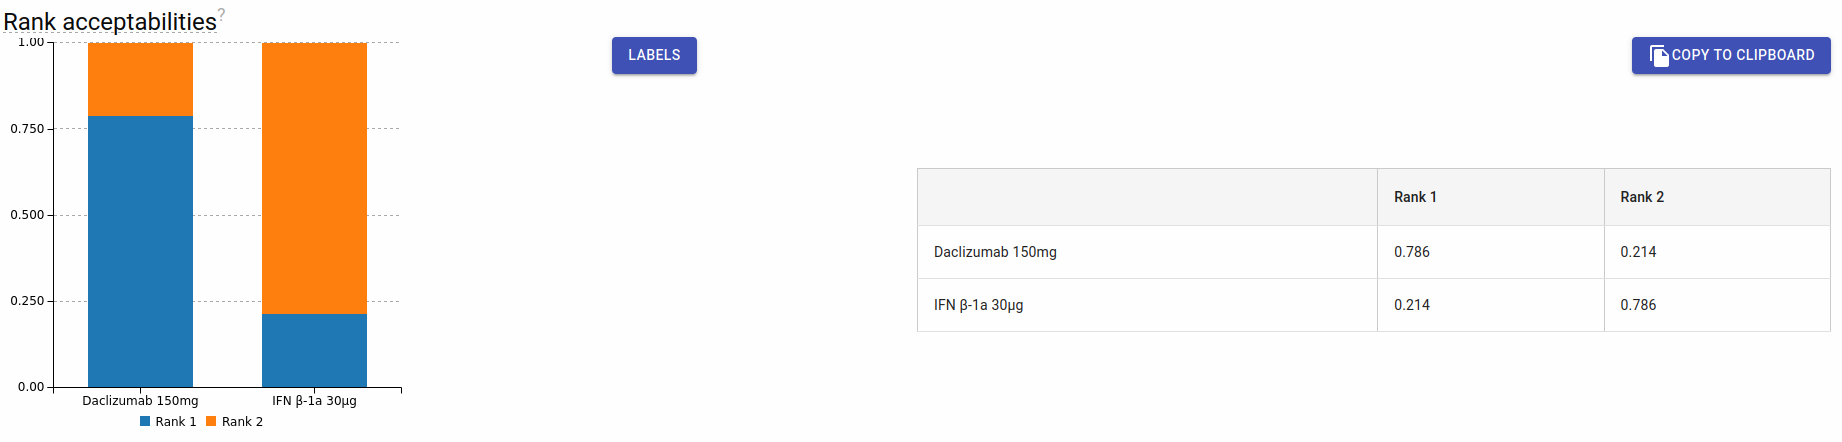
\includegraphics[width=\textwidth]{fig/rankAcceptabilities.png}
    \caption{Rank acceptabilities}
    \label{fig:rankAcceptabilities}
\end{figure}

\noindent \faGraduationCap \, SMAA models explore uncertainties in the measurements and preferences by systematically varying their values\footnotemark. The set of variations (of which there can be hundreds of thousands) can be analysed in several ways. We here use the rank acceptability: for each variation the alternatives are ranked according to their calculated value, and then the proportion of variations in which an alternative had each specific rank is reported.
\footnotetext{SMAA samples from probabilistic distributions for these values - for a more in-depth explanation of the process, see the \href{https://mcda.drugis.org/manual.html}{MCDA manual} and Tervonen \& Lahdelma (2007)}
\newline

\noindent \leftpointright \, Go to the ‘Preferences’ tab, create a new scenario called ‘100-75-50-25’. Set the partial value functions as before, and use Precise Swing to set the Criteria weights as:  ARR 100\%, Hep. AE 75\%, Cut. AE 50\% and Inf. AE 25\%. Go to the ‘Deterministic results’ tab, and you should see that the value of both alternatives is approximately equal. Now navigate to the ‘SMAA’ tab and observe the results. You should see that each alternative is ranked as best in roughly 50\% of all cases. This is consistent with the deterministic analysis, where the value for both alternatives is approximately equal.
\newline

\noindent \leftpointright \, Switch to your workspace from the previous tutorial. Create a scenario in the Preferences tab called ‘ranked weights’, then use Precise swing to specify the weights as:  ARR 100\%, Hep. AE 50\%, Cut. AE 25\% and Inf. AE 12\%. This results in a representative weight distribution approximately equal to the one automatically generated for deterministic analysis of the case where the criteria are ranked.
\newline

\noindent \leftpointright \, Go to the ‘Deterministic results’ tab and use the scenario switching to go back and forth between the ‘ranked weights’ scenario and the ‘Default’ one (assuming you kept that scenario as using ranking; otherwise do a new ranking elicitation). The results and representative weights should be similar.
\newline

\noindent \leftpointright \, Switch to the ‘SMAA results’ tab and again switch back and forth between the two scenarios. Now you should see a great difference. For the specific weight distribution we picked, there is no uncertainty in either the measurements or the preferences, and thus all scenarios result in the same ranking. However, in the ‘Default’ scenario where only ranks are specified, the different ways in which the weights can be distributed while preserving their ranking are taken into account, showing that for only approximately half such rankings Daclizumab 150mg is better than IFN $\beta$-1a 30$\mu$g.
\newline

\noindent \faGraduationCap \, Uncertainty can also lie in the preferences. If only a ranking is specified, there are infinitely many ways to pick the actual weight values for the criteria that still satisfy the given ranking. SMAA also varies the preferences if there is uncertainty there.

\subsection*{Final words}
This tutorial showed how to explore potential consequences of uncertainty in your measurements and preferences for the benefit-risk balance. It also demonstrated how to determine the sensitivity of the benefit-risk balance to changes in measurements and preferences. Finally, we’ve shown how to interpret the output of SMAA models and their bird’s eye view of what is possible.

\end{document}
